%%%%%%%%%%%%%%%%%%%%%%%%%%%%%%%%%%%%%%%%%%%%
% Chapitre 4
%%%%%%%%%%%%%%%%%%%%%%%%%%%%%%%%%%%%%%%%%%%%

\chapter{Méthode linéaire}
\label{Chapter4}

Ce chapitre présente les méthodes de détection développées au cours de la thèse.
De manière classique, la comparaison de groupes en ITD s'effectue sur les cartes scalaires dérivées des images de tenseus, 
comme les cartes de \fa (FA) ou de \md (DM) via le logiciel SPM\footnote{\url{http://www.fil.ion.ucl.ac.uk/spm/}}.
Cependant, chaque indice scalaire caractérise une seule et unique information sur la diffusion.
Ainsi, les autres informations sur la diffusion ne sont pas prises en compte dans le modèle scalaire.
Par contre, les six éléments du tenseur englobent toute l'information de la diffusion.
C'est dans l'optique d'éviter cette perte d'information que nous avons proposés de nouvelles méthodes 
qui sont des extensions de la méthode classique aux images du tenseurs de diffusion.
Elles sont basées sur le \mlg (MLG) et consistent en une régression multi-linéaire suivi d'un test statistique.
Le MGL consiste à représenter les données comme des combinaisons linéaires de variables explicatives et de valeurs d'intérêt, nommés régresseurs à  estimer.
À partir de ces régresseurs, un test statistique nous permet de savoir si ils sont statistiquement différents.
Dans ce chapitre, les notations mathématiques seront les suivantes : $a$ est une variable, $\{a_i\}_{i=1..N}$ est un ensemble de $N$ variables, 
$\mathbf{a}$ est une matrice ou un vecteur, $\hat{a}$ est l'estimée de la variable.
De plus, les régressions multi-linéaires présentées utilisent les métriques du domaine Euclidien.
Le chapitre suivant étudie l'impact des différentes métriques (Euclidiennes, Log-Euclidiennes et Riemanniennes) sur la comparaison de groupes.\\

% \minitoc

%----------------------------------------------------------------------------------------

\section{Régression multi-linéaire}
Cette première section est une introduction au formalisme mathématique de la régression multi-linéaire.
L'expression de \mlg est présentée ainsi que l'étape d'estimation des régresseurs par la méthode des moindres carrés.
Mathématiquement, le concept de régression multi-linéaire peut être décrit de la manière suivante :\\
\begin{adjustwidth}{1cm}{}
    Soit $\mathbb{M}$ une variété et $\{y_i\}_{i \in [1..N]} \in \mathbb{M}$ les observations de $N$ individus pouvant être caractérisés 
    par $K$ variables explicatives (ou covariables) $\{x_{i,j}\}_{j \in [1..K]} \in \mathbb{R}$ telles que l'âge, le genre ou l'affiliation aux différents groupes.
    La régression consiste à estimer une fonction $f : \mathbb{R}^{K} \mapsto \mathbb{M}$ 
    qui fait correspondre au mieux les différents couples $(\{x_{i,1} \dots x_{i,K} \} ,y_i)$
    en minimisant les résidus $\varepsilon_i = y_i - f(\{x_{i,1} \dots x_{i,K} \})$. 
    Pour cela, le modèle utilise des métriques définis sur la variété $\mathbb{M}$.\\
\end{adjustwidth}

Notons que la variété $\mathbb{M}$ peut être : le domaine Euclidien ($\mathbb{M} \subset \mathbb{R}$), le domaine Log-Euclidien ($\mathbb{M} \subset \mbox{Sym}(3)$) 
ou encore le domaine Riemannien ($\mathbb{M} \subset \mbox{Sym}^+(3)$).
Dans cette section, les observations appartiennent à la variété Euclidenne $\mathbb{M} \subset \mathbb{R}$.
Une étude sur l'impact du choix de la variété des métriques sur les résultats de la comparaison de groupes est présentée au \chapref{Chapter5}.

\subsection{Expression du \mlg : $\mathbb{M} \subset \mathbb{R}$}
Le \mlg est un outil fondamental dans les analyses statistiques d'observations.
Il permet d'expliquer les observations avec des variables explicatives en les mettant sous forme de système linéaire
à résoudre $\mathbf{y} = \mathbf{Ax}$.
Deux cas de figures différents sont possibles : le premier cas où les observations sont des scalaires, alors la régression est dite univariée, 
et le second cas qui correspond à une régression multivariée, c'est-à-dire que les observations sont des vecteurs.
Les deux cas d'observations sont présentés dans les paragraphes suivants.
Malgrès cette différence dans les modèles, ils font tous les deux l'hypothèse forte que les résidus $\varepsilon_i$ sont identiquement distribués 
et indépendants $\varepsilon_{i} \overset{idd}{\sim} \mathcal{N}(0, \sigma^2)$ avec $\sigma^2$ la variance du bruit additif du modèle.
De plus, la méthode d'estimation des variables d'intérêt est la même et sera présentée dans la sous-section suivante.

\subsubsection*{Cas d'observations univariées}
Dans la cas d'observations univariées, le \mlg (MLG) permet de représenter une observation $y_{i=1..N} \in \mathbb{R}$, 
comme une combinaison linéaire des variables explicatives $\{x_{i,j}\}_{j \in [1..K]} \in \mathbb{R}$ 
et des variables d'intérêt, les régresseurs $\{\beta_j\}_{j \in [1..K]}$:
\begin{alignat}{2}
    f &:\ \mathbb{R}^{K} &&\mapsto \mathbb{R} \nonumber \\
    &{}\left[\begin{array}{c}
x_{1}\\
\vdots\\
x_{K}
\end{array}\right] &&\mapsto y_i = \beta_{1}x_{i,1} + \beta_{2}x_{i,2} + \dots + \beta_{K}x_{i,K} + \varepsilon
\label{glm}
\end{alignat}
Les différents paramètres à estimer de l'équation \eqref{glm} sont les coéfficients des régresseurs $\{\hat{\beta}\}$.
Chaque régresseur est associé avec une variable explicative et représente l'effet de cette covariable sur l'observation.
Un exemple classique de covariable pour les maladies dégénératives du système nerveux central chez l'homme est celui de l'âge. 
Lorsque un groupe de sujets sains est comparé avec un groupe de sujets atteints d'une pathologie neurodégénérative, 
l'atrophie cérébrale dûe à l'âge des individus peut apparaîre comme régions pathologiques, or elles ne sont pas nécessairement représentatives de la maladie étudiée.
Pour éviter cela, la variable de l'âge est incluse dans le système et permet au modèle d'expliquer une partie de l'observation par cette covariable.

L'estimation du résidu du modèle, représenté par la variable $\varepsilon$, 
découle de celle des régresseurs $\hat{\varepsilon} = y - \hat{\beta_{1}}x_{i,1} + \dots + \hat{\beta_{K}}x_{i,K} $.
Si les variables explicatives ont une distribution centrée alors il faut imposer $x_{1} = 1$ 
(dans la suite du manuscrit, nous considèrerons que nous sommes dans cette configuration).
Un exemple simple de régression multi-linéaire sur un cas univarié
est illustré par la \figref{regression_2D} dans le cas 2D ($K=2$).
Sur la figure, les points bleus correspondent aux couples $(\{1, x_{i,2}\},y_i)$ et la droite affine rouge représente la fonction $f(\{1, x_{i,2}\})$.\\
\begin{figure}[ht]
    \centering
    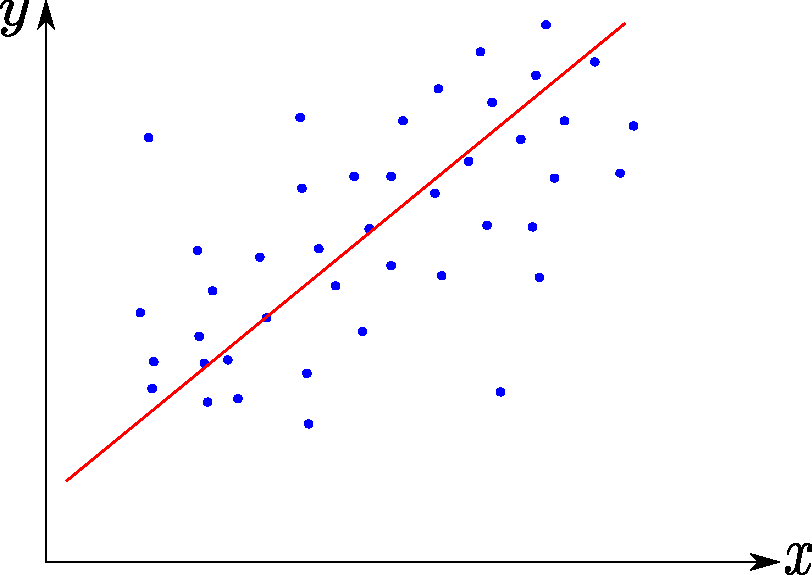
\includegraphics[scale=0.5]{Images/regression_2d.pdf}
    \caption{\label{regression_2D} Illustration d'une régression multi-linéaire 2D ($K=2$). 
    Les points bleus correspondent aux couples $(\{1, x_{i,2}\} ,y_i)$ et la droite affine rouge à la fonction $f(\{1, x_{i,2}\})$.}
\end{figure}

Dans le cas multi-linéaire d'un modèle avec $N$ observations,
l'équation \eqref{glm} peut facilement s'écrire sous la forme matricielle.
Les observations sont stockés dans le vecteur $\mathbf{Y} = \left[y_1\dots y_i\dots y_N\right]^{t}$, 
les variables explicatives associées aux observations dans la matrice $\mathbf{X}\left[i,j\right] = x_{i,j} \mbox{ avec } \mathbf{X}\left[i,0\right] = 1$,
les régresseurs sont dans le vecteur $\mathbf{B} =\left[\hat{\beta_{1}}\dots \hat{\beta_j}\dots \hat{\beta_K}\right]^{t}$.
et les résidus dans le vecteur $\mathbf{e} = \left[\varepsilon_1\dots \varepsilon_i\dots \varepsilon_N\right]^{t}$. 
Avec ce modèle, les résidus suivent tous la même distribution $\mathbf{e} \overset{idd}{\sim} \mathcal{N}(0, \sigma^2)$.
\begin{equation}
    \underbrace{\mathbf{Y}}_{N\times 1} = 
	      \underbrace{\mathbf{X}}_{N\times K}\underbrace{\mathbf{B}}_{K\times 1} + \underbrace{\mathbf{e}}_{N\times 1}
    \label{glm_mat}
\end{equation}

\subsubsection*{Cas d'observations multivariées}
Dans le cas dit \og mutlivariées \fg, pour chaque individu, les observations sont des vecteurs $\{y_{i,m}\}_{m=1..M} \in \mathbb{R}$ 
et les variables explicatives $\{x_{i,j}\}$ sont les mêmes pour chaque élément du vecteur.
Ainsi l'équation \eqref{glm} peut être réécrite de la manière suivante :
\begin{alignat}{2}
    f &:\ \mathbb{R}^{K} &&\mapsto \mathbb{R}^{N}\times\ \mathbb{R}^{M} \nonumber \\
    &{}\left[\begin{array}{c}
x_1\\
\vdots\\
x_K
\end{array}\right] &&\mapsto \left[\begin{array}{c}
\mathbf{y_1} = \left[y_{1,1} \dots y_{1,m} \dots y_{1,M} \right]\\
\vdots\\
\mathbf{y_N} = \left[y_{N,1} \dots y_{N,m} \dots y_{N,M} \right]
\end{array}\right]
\label{glm_multi}
\end{alignat}

Pour chaque élément des vecteurs, le \mlg décompose les données comme une combinaison linéaire des variables explicatives associées à l'individu
et des régresseurs associés à l'élément du vecteur :

\begin{align}
    y_{1,m} &= \beta_{1,m}x_{1,1} + \beta_{2,m}x_{1,2} + \dots + \beta_{K,m}x_{1,K} + \varepsilon_{1,m} \nonumber\\
    y_{i,m} &= \beta_{1,m}x_{i,1} + \beta_{2,m}x_{i,2} + \dots + \beta_{K,m}x_{i,K} + \varepsilon_{i,m} 
\end{align}

Ce système se traduit en écriture matricielle pour le $m^\text{ème}$ élément du vecteur d'observation par l'équation \eqref{glm_mat_multi}. 
Ce modèle est équivalent à $M$ modèles univariés indépendants, un pour chaque composante $m$ des vecteurs d'observation 
avec la même matrice de dessin $\mathbf{X}$ que pour le cas univarié.

\begin{equation}
     \underbrace{\mathbf{Y_m}}_{N\times 1} = 
	      \underbrace{\mathbf{X_{}}}_{N\times K}\underbrace{\mathbf{B_m}}_{K\times 1} + \underbrace{\mathbf{e_m}}_{N\times 1}
    \label{glm_mat_multi}
\end{equation}

Le modèle représentant les performances académiques d'étudiants est un exemple simple pour illustré le cas d'observations multivariées.
Prenons une étudiante $i$ avec ses moyennes pour les deux sessions de partiels semestriels $y_{i,1} \mbox{ et } y_{i,2}$.
Sachant le nombre d'heure qu'elle a passé à étudier par semaine $x_{i,2}$, son QI $x_{i,3}$ et son rang de l'année précédente $x_{i,4}$, 
le mlg permet d'écrire un système pour $K=4$ variables explicatives (avec $x_{i,1} = 1$):

\begin{equation}
    \mathbf{y_i} =
    \left[\begin{array}{c}y_{i,1}\\y_{i,2}\end{array}\right] = 
    \left[\begin{array}{c}\beta_{1,1} + \beta_{2,1}x_{i,2} + \beta_{3,1}x_{i,3} + \beta_{3,1}x_{i,3} + \varepsilon_{i,1}\\
			  \beta_{1,2} + \beta_{2,2}x_{i,2} + \beta_{3,2}x_{i,3} + \beta_{3,2}x_{i,3} + \varepsilon_{i,2}\end{array}\right] \nonumber
\end{equation}

Pour une promotion entière composée de $N$ étudiants, le \mlg permet de représenter deux systèmes ($M=2$) de régression multi-linéaire \eqref{ex_glm_multi}.
Avec ce modèle, les deux vecteurs de résidus suivent deux lois normales différentes $\mathbf{e_m} \overset{idd}{\sim} \mathcal{N}(0, \sigma^2_m)$.

\begin{align}
    \mathbf{Y_1} = \mathbf{X}\mathbf{B_1} + \mathbf{e_1} \nonumber \\
    \mathbf{Y_2} = \mathbf{X}\mathbf{B_2} + \mathbf{e_2} 
    \label{ex_glm_multi}
\end{align}


\subsection{Estimation des régresseurs : la méthode des moindres carrés}
Le \mlg met en place un système linéaire à résoudre $\mathbf{Y} = \mathbf{XB}+\mathbf{e}$. 
Il représente les observations comme une combinaison linéaire de variables explicatives 
et de variables d'intérêt avec un bruit additif gaussien $\varepsilon_{i} \overset{idd}{\sim} \mathcal{N}(0, \sigma^2) \label{res_iid}$.
Pour résoudre ce système, il faut estimer les $K$ variables d'intérêt  $\{\beta_{j}\}_{j=1..K}$.
Le meilleur estimateur au sens du maximum de vraisemblance pour des observations avec un bruit additif gaussien est l'estimateur par la méthode les moindres carrés.
La méthode proprose de minimiser l'erreur quadratique entre les observations et la combinaison linéaire pour estimer les régresseurs $\{\hat{\beta}_{j}\}_{j=1..K}$.
\begin{align}
    \mathbf{\hat{B}} &= \arg\min_{B \in \mathbb{R}^{k}}{\|\mathbf{Y} - \mathbf{X}\mathbf{B} \|^{2}} \nonumber\\
     &= (\mathbf{X}^{t}\mathbf{X})^{-1}\mathbf{X}^{t}\mathbf{Y}
    \label{ls_reg}
\end{align}

Les propriétés asymptotiques de l'estimateur par les moindres carrés sont connues 
et le fait que les résidus du modèle suivent une distribution normale implique 
que les régresseurs suivent une loi de gaussienne de moyenne $E(\mathbf{B}) = \mathbf{\hat{B}}$ et de variance $Cov(\mathbf{B}) = \mathbf{\hat{\varSigma}}$
\begin{equation}
    \mathbf{B} \sim \mathcal{N}(\mathbf{\hat{B}}, \mathbf{\hat{\varSigma}})
\end{equation}
L'expression analytique de l'estimée de $\mathbf{\hat{B}}$ est donnée par l'équation \eqref{ls_reg} et $\mathbf{\hat{\varSigma}}$ peut en être directement déduite :
\begin{align}
    \mathbf{\hat{\varSigma}} &= \hat{\sigma}^{2}(\mathbf{X}^{t}\mathbf{X})^{-1} \label{ls_reg_VAR}\\
    \text{avec } \hat{\sigma}^{2} &= \frac{1}{N-K}\|\mathbf{Y} - \mathbf{X}\mathbf{\hat{B}} \|^{2} \label{ls_reg_var}
\end{align}

Dans le cas d'observations multivariées, il faut faire une estimation par les moindres carrés pour chaque équation du système \eqref{ex_glm_multi}.

\subsection{Exemple d'application aux images de scalaires}
Ce paragraphe est un exemple d'application du \mlg avec des observations univariées.
Il correspond à la méthode classique employée par SPM pour faire une comparaison de groupes en ITD sur des images de scalaires dérivées des images de tenseurs de diffusion.

Soit $N$ le nombre d'individus total divisé en deux groupes avec respectivement $N_1$ sujets sains et $N_2$ sujets atteints d'une pathologies.
L'observation $y_i$ représente la valeur d'un voxel $p$ de l'image de scalaire (par exemple l'image de \fa FA) pour le $i\text{ème}$ individu.
L'ensemble des observations $\{y_i\}_{i=1..N}$ correspond aux valeurs du voxel $p$ de tous les $N$ individus.

\begin{equation}
    \underbrace{\mathbf{Y}_{}}_{N\times 1} = \left[\begin{array}{c}
                                             y_1\\
                                             \vdots\\
                                             y_N
                                         \end{array}\right]
  \xrightarrow{\text{correspond à}} 
  \underbrace{\mathbf{Y}_{}^p}_{N\times 1} = \left[\begin{array}{c}
                                             FA_1^p\\
                                             \vdots\\
                                             FA_N^p
                                         \end{array}\right]
\end{equation}

Soit $K=3$ variables explicatives associées au modèle :
$x_{1,\cdot}=1$ est la constante de \og centrage \fg, 
$x_{2,\cdot}= \{0,1\}$ la covariale d'affiliation au groupe ($0$ si l'individu appartient au groupe sain et $1$ s'il appartient au groupe atteint)
et $x_{3,\cdot}$ la variable de l'âge.
La matrice de dessin s'écrit donc de la manière suivante.

$$\underbrace{\mathbf{X}_{}}_{N\times K} = \left[\begin{array}{ccc} 
                                             centre & gp & \hat{a}ge\\
                                             1 & 0 & 36\\
                                             1 & 0 & 28\\
                                             \vdots & \vdots & \vdots\\
                                             1 & 1 & 25\\
                                             1 & 1 & 37\\
					      \end{array}\right] $$

Grâce à la $2^{\text{ième}}$ covariable (celle du groupe), le \mlg permet de quantifier l'effet du groupe sur les observations. 
Ainsi, pour un voxel $p$ donné, il est possible d'évaluer si il appartient statistiquement plus au groupe sain ou au groupe atteint.
Par exmple, si un axone (passant par le voxel $p$) est dymélinisé par la pathologie
alors la valeur de la FA en ce voxel sera moins élévée que celle du voxel sain sans démyélinisation.
Ce voxel aura alors une forte probabilité d'être représentatif de la maladie.
La covariable de l'âge permet de corriger les effets dûs au vieillissement naturel du cerveau dans le modèle.
Il est également possible de voir cet effet de l'âge sur le cerveau en analysant le régresseur associé.

Il est intéressant de voir qu'il est inutile de résoudre un seul système \eqref{glm_mat} par voxel.
Une concaténation de toutes les valeurs des $V$ voxels dans la matrice $\mathbf{Y}$ est possible.
Cela permet d'estimer les $K$ régresseurs de chaque voxel en une seule et unique opération de pseudo-inverse.
\begin{equation}
    \underbrace{\mathbf{Y}}_{N\times V} = 
	      \underbrace{\mathbf{X}}_{N\times K}\underbrace{\mathbf{B}}_{K\times V} + \underbrace{\mathbf{e}}_{N\times V}
    \label{ex_glm_mat}
\end{equation}



\section{Cadre statistique}
Le test statistique est la deuxième étape de la comparaison de groupes.
Il permet de quantifier les effets des régresseurs de manière statistique pour chaque voxel de l'image.
Un effet est dit significatif si il traduit un réel écart entre les deux groupes, et permet ainsi de conclure à l'existence d'une différence.
Pour cela, un test d'hypothèse est défini, permettant de formuler une règle de décision pour statuer si la différence est significative ou si elle ne l'est pas.
Cette prise de décision est basée sur la notion d'erreur associée à une probabilité donnée par le résultat du test statistique.

\subsection{Tests d'hypothèse}
Un test d'hypothèse est un test statistique qui permet d'associer une valeur à une prise de décision dans le but de quantifier la confiance en une hypothèse.
Deux hypothèses peuvent être formulées dans un cadre statistique :\\
\begin{itemize}
    \item l'hypothèse nulle $\mathcal{H}_{0}$ qui exprime une absence d'effet. 
    Cela se traduit par le fait que pour un régresseur donné, il n'y a aucune différence significative entre les deux groupes. 
    Les écarts observés sont dûs au bruit et à la variabilité inter-individus.
    Suivant les résultats du test statistique, l'hypothèse nulle $\mathcal{H}_{0}$ est acceptée ou rejetée.\\
    \item l'hypothèse de rejet $\mathcal{H}_{1}$ qui représente l'hypothèse alternative si $\mathcal{H}_{0}$ est rejetée.\\
\end{itemize}

Dans le contexte de comparaison de groupes en imagerie médicale pour un voxel, l'hypothèse nulle définit $\mathcal{H}_{0}$\textit{ : aucun changement significatif}
et l'hypothèse alternative $\mathcal{H}_{1}$\textit{ : changement détecté significatif}.

\subsection{Règle de décision}
Dans ce cadre statistique, il y a deux vérités et deux décisions possibles, ce qui conduit à quatre configurations différentes (voir \tabref{tab_test_hypo}).
Elles entrainent deux types d'erreur qui sont les erreurs de première $\alpha$ et de deuxième $\beta$ espèce (voir \figref{loi_norm}).\\
\begin{itemize}
    \item la vérité correspond à l'hypothèse nulle $\mathcal{H}_{0}$ et le test accepte cette hypothèse. 
    Cela mène à une bonne détection avec une probabilité de $1-\alpha$, ou encore la probabilité d'avoir un Vrai Négatif ($VNeg$).\\
    \item la vérité est l'hypothèse nulle $\mathcal{H}_{0}$ et le test rejette cette hypothèse.
    Cela correspond à détecter un Faux Positif ($FPos$) avec une probabilité de $\alpha$.\\
    \item la vérité est l'hypothèse $\mathcal{H}_{1}$ et le test accepte cette hypothèse.
    Cette configuration mène à une bonne décision par la détection d'un Vrai Positif ($VPos$) avec une probabilité de $1-\beta$.\\
    \item la vérité est l'hypothèse $\mathcal{H}_{1}$ et le test rejette cette hypothèse.
    Ce cas correspond à la probabilité $\beta$ d'avoir un Faux Négatif ($FNeg$).\\
\end{itemize}

\begin{table}[ht]
  \centering
  \begin{tabular}{|c|c|c|}
      \hline
      \diagbox{Décision}{Vérité} & $\mathcal{H}_{0}$ & $\mathcal{H}_{1}$ \tabularnewline
      \hline
      $\mathcal{H}_{0}$ & $1-\alpha\ (VNeg)$ & $\beta\ (FNeg)$ \tabularnewline
      $\mathcal{H}_{1}$ & $\alpha\ (FPos)$ & $1-\beta\ (VPos)$ \tabularnewline
      \hline
  \end{tabular}
  \caption{\label{tab_test_hypo}Choix possibles lors de la décision : probabilité d'accepter ou de rejeter l'hypothèse $\mathcal{H}_{0}$ 
	    exprimée par l'erreur de première espèce $\alpha$ et de deuxième espèce $\beta$.
	    Les probabilités sont associées aux types de détections {$VNeg$, $VPos$, $FPos$, $FNeg$} correspondant respectivement 
	    aux nombres de Vrais Négatifs, Vrais Positifs, Faux Postitifs et Faux Négatifs.} 
\end{table}
\begin{figure}[ht]
    \centering
    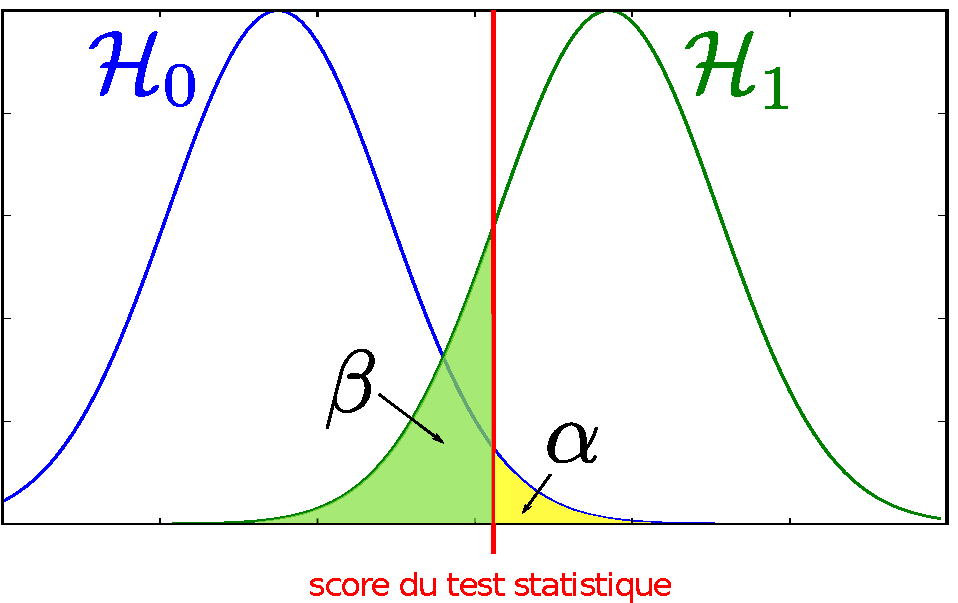
\includegraphics[scale=0.5]{Images/loi_norm.pdf}
    \caption{\label{loi_norm}Illustration des erreurs de première $\alpha$ et de deuxième $\beta$ espèce.}
\end{figure}

Il existe deux types de tests d'hypothèse : 
les tests paramétriques pour lesquels la loi de probabilité sous l'hypothèse $\mathcal{H}_{0}$ est connue ($f_0$)
et les tests non-paramétriques pour lesquels elle n'est pas connue.
En règle générale, la distribution sous l'hypothèse $\mathcal{H}_{1}$ n'est pas connue et ne peut pas être modèlisée.
Un état de l'art sur les différents tests paramétriques et non-paramétriques en détection de changements en imagerie de diffusion
est présenté dans le manuscrit de thèse \cite{Grigis_PhD}.\\

Dans le cas des tests paramétriques, il est possible de calculer une probabilité, nommée \textit{p-valeur} (voir \figref{calcul_p_valeur}), associée à une valeur statistique ($s$) du test.\\
\begin{equation}
    \text{\textit{p-valeur}} = \int_{seuil}^{\infty} f_0(s)ds
\end{equation}

\begin{figure}[ht]
    \centering
    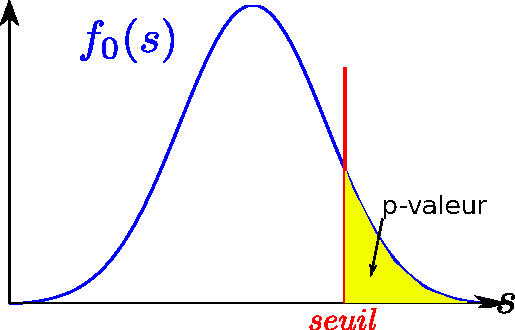
\includegraphics[scale=0.6]{Images/calcul_p_valeur.pdf}
    \caption{\label{calcul_p_valeur}Calcul de la p-valeur : 
    aire sous la courbe $f_0(s)$ représentant la distribution sous l'hypothèse $\mathcal{H}_{0}$ pour une valeur statistique du test ($seuil$).}
\end{figure}

À partir de l'erreur de première espèce $\alpha$ ou de la \textit{p-valeur}, deux façons de procéder sont possibles.
La première consiste à imposer la valeur de l'erreur $\alpha$ et à calculer la valeur statistique ($seuil$) associée en fonction de la loi $f_0$.
Ensuite, l'hypothèse est acceptée ou rejetée si le résultats du test est, respectivement, inférieur ou supérieur à ce $seuil$.
La deuxième stratégie commence d'abord à calculer la \textit{p-valeur} associée à la valeur statistique ($seuil$) en fonction de la loi $f_0$
pour après la comparer avec la valeur souhaitée de l'erreur $\alpha$.\\

Dans le cas des tests non-paramétriques, la loi de probabilité sous l'hypothèse $\mathcal{H}_{0}$ est inconnue, 
rendant impossible la modélisation de la distribution et le calcul de \textit{p-valeur}.
Il est néanmoins possible d'estimer la fonction $f_0$ en utilisant une méthode de permutation introduite par \cite{Chung2008}.
De manière générale, une permutation correspond à une interversion de deux valeurs de la matrice dessin $x_{i_{1},j}$ et $x_{i_{2},j}$,
$j$ étant à la variable d'intérêt (par exemple le groupe).\\
\begin{equation}
    \underbrace{
	  \left[\begin{array}{ccc} 
	  centre & gp & \hat{a}ge\\
	  1 & 0 & 36\\
	  1 & 0 & 28\\
	  \vdots & \vdots & \vdots\\
	  1 & 1 & 25\\
	  1 & 1 & 37\\
	  \end{array}\right]
      \ldots
	  \left[\begin{array}{ccc}
	  centre & gp & \hat{a}ge\\
	  1 & 1 & 36\\
	  1 & 0 & 28\\
	  \vdots & \vdots & \vdots\\
	  1 & 1 & 25\\
	  1 & 1 & 37\\
	  \end{array}\right]
      \ldots 
	  \left[\begin{array}{ccc}
	  centre & gp & \hat{a}ge\\
	  1 & 0 & 36\\
	  1 & 0 & 28\\
	  \vdots & \vdots & \vdots\\
	  1 & 0 & 25\\
	  1 & 1 & 37\\
	  \end{array}\right]
	  }_{T\ permutations} \nonumber
\end{equation}

La méthode de permutation consiste à calculer les scores du test non-paramétrique proposé pour $T$ permutations différentes.
L'histogramme de tous les scores obtenus permet d'estimer la loi de distribution sous $\mathcal{H}_{0}$.
À partir de cet histogramme et d'un niveau de significance $\alpha$ choisi, 
le calcule du score $seuil$ du test statistique (première stratégie présentée dans le paragraphe précédent) devient possible.
L'importance du nombre $T$ de permutations est évidente : pour $T=1000$ permutations, la plus petite \textit{p-valeur} est $0.001$. 
Pour avoir une plus grande précision, il faut donc augmenter le nombre de permutations.
Un inconvénient majeur à cette méthode est le temps de calcul qu'elle génére.
En comparaison, un test paramétrique effectue une opération alors que un test non-paramétrique va effectuer cette opération $T$ fois.

\subsection{Test statistique de comparaison utilisé}
Dans nos études, un test statistique de Fisher est utilisé pour évaluer si une des variables explicatives contribue de manière significative dans le modèle de régression.
Pour cela, le test compare, au sens des moindres carrés, les résidus de deux modèles imbriqués : 
un modèle dit \og complet \fg qui prend en compte toutes les variables explicatives ($\mbox{RSS}_{2}$)
et un modèle dit \og restreint \fg où la covariable d'intérêt est rejeté ($\mbox{RSS}_{1}$) :
\begin{equation}
    F = \frac{\displaystyle \frac{RSS_{1} - RSS_{2}}{\displaystyle p_{2} - p_{1}} }{\displaystyle \frac{RSS_{2}}{ \displaystyle N - p_{2}}}
    \label{test_stat}
\end{equation}
avec $ p_{2} \mbox { et } p_{1}$, représentant respectivement le nombre de variables explicatives des deux modèles et $N$ le nombre d'observations.
En supposant que les résidus suivent une distribution normale ($\varepsilon \sim \mathcal{N}(0, \sigma^2)$), 
$F$ suit une distribution de Fisher avec $p_{2}-p_{1}$ et $ N-p_{2} $ degrés de liberté,
sous l'hypothèse nulle $\mathcal{H}_{0}$ que le modèle 2 ne fournit pas un meilleur ajustement des variables explicatives aux données que le modèle 1.

L'hypothèse gaussianité des résidus est une hypothèse raisonnable dans un cadre Euclidien et Log-Euclidien mais elle n'est plus valable pour un cadre Riemannien.
Dans ce dernier cas, pour obtenir des cartes de \textit{p-valeur}, une méthode de permutation peut être utilisée mais cela demande des temps de calcul prohibitifs.


\section{Extension du \mlg aux tenseurs}
Dans la section précédente, nous avons montré un exemple d'application du \mlg aux images de Fraction d'Anisotropie.
Cette méthode fournit des résultats seulement sur des changements spécifiques à la FA.
Il manque, dans ce modèle, des informations sur la diffusion pour détecter tous les types de changements existants,
par exemple changements de diffusion moyenne ou encore modification d'orientation.
Ces informations multiples qui permettent de caractériser de manière générale la diffusion sont toutes contenues dans le tenseur de diffusion.
C'est dans cet optique de ne perdre aucnue information que nous avons développé une méthode basée sur le \mlg 
pouvant être appliquée sur des images de tenseur de diffusion.

Dans notre extension du \mlg aux tenseurs de diffusion, nous avons considéré trois stratégies : 
les deux premières sont basées sur des hypothèses d'homoscédasticité et d'hétéroscédasticité des données alors que
la dernière utilise l'information présente dans le voisinage du voxel analysé.
La première stratégie est un cas de \mlg avec des observations univariées alors que les deux autres utilisent des données mutlivariées.
Pour rappel, le tenseur $\mathbf{D}$ est un matrice symétrique définie positive de dimension 3.
Dans cette section, elle est exprimée comme un vecteur des six éléments supérieurs de la matrice :
$$vect\ (\mathbf{D})=\left[D_{xx}\ D_{xy}\ D_{xz}\ D_{yy}\ D_{yz}\ D_{zz}\right]^{t}$$

\subsection{Hypothèse d'homoscédasticité}
L'hypothèse d'homoscedasticité consiste à supposer que la variance du bruit de chaque élément du tenseur $D_{\largedot\largedot}^i$ est identique :
$\varepsilon_i \sim \mathcal{N}(0, \sigma^2)$.
Ce modèle se présente sous la même forme que le \mlg pour un cas d'observations univariées.
Pour prendre en compte toutes les informations liées à la diffusion, 
les six éléments du tenseur $\mathbf{D^i}$ du $i^\text{ème}$ sujet sont concaténés en un seul vecteur vertical 
$vec\ (\mathbf{D^i})=\left[D^i_{xx}\ D^i_{xy}\ D^i_{xz}\ D^i_{yy}\ D^i_{yz}\ D^i_{zz}\right]^{t}$  
et chaque élément du tenseur est considéré une observation.
Le modèle précédent passe donc de $N$ observations à un modèle composé de $N\times 6$ observations.

\begin{equation}
    \underbrace{\mathbf{Y}_{}}_{N\times 1} = \left[\begin{array}{c}
                                             y_1\\
                                             \vdots\\
                                             y_N
                                         \end{array}\right]
  \xrightarrow{\text{devient}}
  \underbrace{\mathbf{Y}_{}}_{(N\times 6)\times 1} = \left[\begin{array}{c}
                                             D^1_{xx}\\
                                             D^1_{xy}\\
                                             D^1_{xz}\\
                                             D^1_{yy}\\
                                             D^1_{yz}\\
                                             D^1_{zz}\\
                                             \vdots\\
                                             D^N_{xx}\\
                                             D^N_{xy}\\
                                             D^N_{xz}\\
                                             D^N_{yy}\\
                                             D^N_{yz}\\
                                             D^N_{zz}\\
                                         \end{array}\right]
\end{equation}

Les observations sont une combinaison linéaire des $K$ variables explicatives (âge, sexe, affiliations, score clinique ...).
Pour chaque variable explicative, six régresseurs sont estimés, un associé à une composante du tenseur.
Cela est fait en construisant une nouvelle matrice de dessin $X\left[i,j\right] = x_{i,j}\text{ pour } i = 1\dots N\times 6\text{ et } j=1\dots K \times 6$
où chaque variable explicative est répliquée en six colonnes.
Pour faire cela, la première colonne est composée des valeurs de la variable explicative pour les entrées correspondant à la première composante du tenseur $D^i_{xx}$ et de zéros pour les autres entrées, et ainsi de suite pour les cinq autres colonnes).

\begin{equation}
    \underbrace{\mathbf{X}_{}}_{N\times K} = \left[\begin{array}{ccc} 
                                             centre & gp & \hat{a}ge\\
                                             1 & 0 & 36\\
                                             1 & 0 & 28\\
                                             \vdots & \vdots & \vdots\\
                                             1 & 1 & 25\\
                                             1 & 1 & 37\\
					      \end{array}\right]
  \xrightarrow{\text{devient}}
  \underbrace{\mathbf{X}_{}}_{(N\times 6)\times (K\times 6)} = \left[\begin{array}{ccc}
								centre & gp & \hat{a}ge\\
								I_{6} & 0_{6} & 36\times I_{6}\\
								I_{6} & 0_{6} & 28\times I_{6}\\
								\vdots & \vdots & \vdots\\
								I_{6} & I_{6} & 25\times I_{6}\\
								I_{6} & I_{6} & 37\times I_{6}\\
								\end{array}\right]
\end{equation}

Avec cette formulation, l'estimation de $\mathbf{B}$ par la méthode des moindres carrés conduit à $K$ régresseurs composés de six éléments, 
chacun associé à un élément du tenseur.
Sans aucune modification sur l'équation \eqref{ls_reg_var}, 
elle permet de calculer directement les résidus du modèle au sens des moindres carrés $RSS = \|\mathbf{Y} - \mathbf{X}\mathbf{\hat{B}} \|^{2}$.
Dans la suite du manuscrit, cette méthode se nommera \mlg Univarié pour les Tenseurs de Diffusion (\textit{MLG-U-TD}).


\subsection{Hypothèse d'hétéroscédasticité}
Cette deuxième hypothèse permet de supposer que le bruit qui affecte chaque composante du tenseur $D_{\largedot\largedot}^i$ 
a une variance différente $\varepsilon_i \sim \mathcal{N}(0, \sigma_{\largedot\largedot}^2)$.
Cette hypothèse semble plus pertinente que l'hypothèse d'homoscedasticité sur les éléments d'un tenseur de diffusion 
si nous regardons (voir \figref{hist_var}) l'histogramme des valeurs de l'estimateur non biaisé de la variance 
présenté par \eqref{ls_reg_var} pour chaque élément des tenseurs d'une image en ITD de dimension $148*148*41$. 
La différence des histogrammes est flagrante.
Les variances des éléments diagonaux ont une répartition assez proche, de même que pour les éléments anti-diagonaux.
Cette histogramme tend à confirmer l'hypothèse d'hétéroscédasticité.

\begin{figure}[ht]
    \centering
    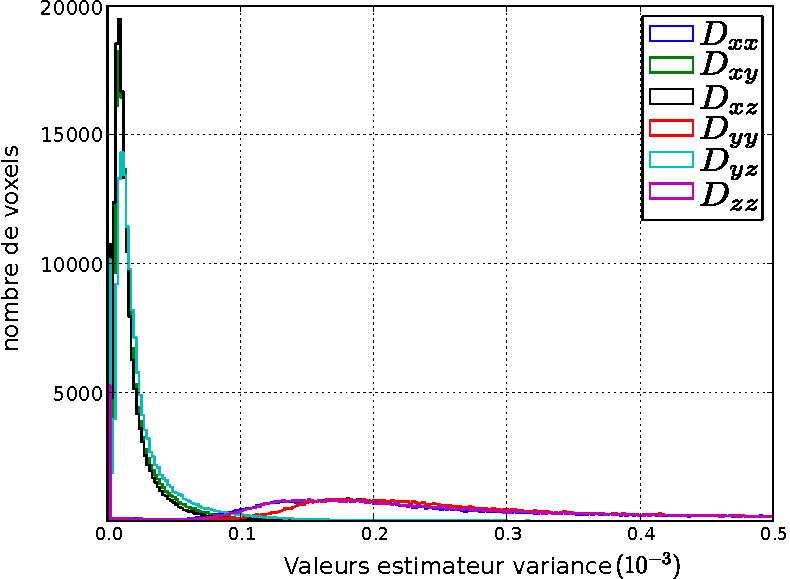
\includegraphics[scale=0.6]{Images/hist_var.pdf}
    \caption{\label{hist_var}Histogrammes des valeurs (en nombres de voxels) de l'estimateur de la variance $\sigma^2$ (en $10^{-3}$)
    pour chaque élément du tenseur.}
\end{figure}

Le modèle sous l'hypothèse d'hétéroscédasticité devient un cas d'observations multivariées 
où les tenseurs représentent les vecteurs d'observations.
La matrice des observations s'écrit alors simplement de la manière suivante :

\begin{equation}
    \underbrace{\mathbf{Y}_{}}_{N\times 1} = \left[\begin{array}{c}
                                             y_1\\
                                             \vdots\\
                                             y_N
                                         \end{array}\right]
  \xrightarrow{\text{devient}}
  \underbrace{\mathbf{Y}_{}}_{(N\times 6)} = \left[\begin{array}{ccccccccccccc}
                                             D^1_{xx} & D^1_{xy} & D^1_{xz} & D^1_{yy} & D^1_{yz} & D^1_{zz}\\
                                              & & & \vdots & & \\
                                             D^N_{xx} & D^N_{xy} & D^N_{xz} & D^N_{yy} & D^N_{yz} & D^N_{zz}\\
                                         \end{array}\right]
\end{equation}

Cette méthode est équivalente à indépendamment estimer six régressions univariées, une pour chaque élément du tenseur, 
avec la même matrice de dessin que pour l'application sur les image de \fa ($X\left[i,j\right] = x_{i,j} \text{, pour } i = 1\dots N \text{ et } j = 1\dots K$). 
Chacune de ses six régressions permet d'estimer les $K$ régresseurs associés à chaque composant du tenseur.
Cela conduit à l'estimation de six résidus au sens des moindres carrés $RSS_{t=1..6}$.
La question qui se pose à cette étape est : Comment fusionner les informations des six résidus $RSS_{t=1..6}$ ?
En effet, si nous appliquons le test de Fisher aux six résidus $RSS_{t=1..6}$, nous obtenons six scores différents.
Comment prendre en compte et quantifier ces six scores correctement ? 
La solution triviale de sélectionner un score (le plus grand ou le plus petit par exemple)
parmi les six valeurs revient à perdre l'apport d'information fourni par la prise e compte de tous les éléments du tenseur.
La méthode de combinaison des probabilités proposée par \cite{Whitlock2005} permet de s'affranchir de ce problème
en présentant un nouveau test fusionnant les \textit{p-valeurs} des six tests de Fisher précédent.\\
\begin{equation}
    z = \frac{\sum_{t=1}^{6} \Phi^{-1}(1-p_t)}{\sqrt{6}} 
    \label{fusion}
\end{equation}
avec $\Phi$ la fonction de répartition et $p_t$ la $t^\text{ième}$ \textit{p-valeur}.
L'équation \eqref{fusion} permet de calculer à nouveau un score qui suit une loi normal
$z\ \overset{iid}{\sim}\ \mathcal{N}(0, 1)$.
Ce test étant paramétrique, il est facile de calculer une nouvelle et unique \textit{p-valeur} représentant les six autres.
Dans la suite du manuscrit, cette méthode se nommera \mlg Multivarié pour les Tenseurs de Diffusion (\textit{MLG-M-TD}).


\subsection{Prise en compte des informations multi-échelles}
Dans les deux méthodes présentées dans les paragraphes précédents, seule l'information contenue dans un voxel est utilisée.
L'idée d'exploiter l'information présente dans les voxels voisins est pertinente et souvent utilisée en traitement d'images médicales \cite{Grigis2012}.
De même que l'idée de prendre en compte l'information du voxel à différentes résolutions : fine, normale et grossière.
Cette dernière façon de faire est utilisée de manière récurrente dans des méthodes de recalage \cite{Yap2009} ou d'extraction de caractéristiques.

Pour ce modèle, la méthode consiste à faire $G=3$ régressions univariées avec une hypothèse d'homoscedasticité sur le vecteur du tenseur. 
Ces régressions prennent comme observations les élements du tenseur avec trois niveaux de filtrages différents : la première utilise les observations brutes sans filtrage, la deuxième utilise un filtre d'une largeur normale (cela correspond au filtrage classique effectué sur les observations avant les deux méthodes précédentes) et la troisième régression utilise un filtrage plus large.
Toutes ces observations sont ensuite concaténées dans une seule matrice $\mathbf{Y}$ (voir équation \eqref{glm_echelle}).

\begin{equation}
    \underbrace{\mathbf{Y}_{}}_{N\times 1} = \left[\begin{array}{c}
                                             y_1\\
                                             \vdots\\
                                             y_N
                                         \end{array}\right]
  \xrightarrow{\text{devient}}
  \underbrace{\mathbf{Y}_{}}_{(N\times 6)\times G} = \left[\begin{array}{ccc}
                                             D^1_{xx} & D^{1,g}_{xx} & D^{1,G}_{xx}\\
                                             D^1_{xy} & D^{1,g}_{xy} & D^{1,G}_{xy}\\
                                             D^1_{xz} & D^{1,g}_{xz} & D^{1,G}_{xz}\\
                                             D^1_{yy} & D^{1,g}_{yy} & D^{1,G}_{yy}\\
                                             D^1_{yz} & D^{1,g}_{yz} & D^{1,G}_{yz}\\
                                             D^1_{zz} & D^{1,g}_{zz} & D^{1,G}_{zz}\\
                                             \vdots & \vdots & \vdots\\
                                             D^N_{xx} & D^{N,g}_{xx} & D^{N,G}_{xx}\\
                                             D^N_{xy} & D^{N,g}_{xy} & D^{N,G}_{xy}\\
                                             D^N_{xz} & D^{N,g}_{xz} & D^{N,G}_{xz}\\
                                             D^N_{yy} & D^{N,g}_{yy} & D^{N,G}_{yy}\\
                                             D^N_{yz} & D^{N,g}_{yz} & D^{N,G}_{yz}\\
                                             D^N_{zz} & D^{N,g}_{zz} & D^{N,G}_{zz}\\
                                         \end{array}\right]
  \label{glm_echelle}
\end{equation}

Par la suite, cette méthode est identique à celle avec l'hypothèse d'hétéroscédasticité. 
De la même manière, les $G$ \textit{p-valeurs} sont combinées par la méthode \cite{Whitlock2005}.
Elle sera nommée \mlg avec Voisinage pour les Tenseurs de Diffusion (\textit{MLG-V-TD}) dans la suite du document.

